\documentclass[sigconf,letterpaper]{acmart}

% For citations having Chinese characters in the title
\usepackage{CJKutf8}

% For tables
\usepackage{multirow}
\usepackage{booktabs}

% Don't use monospace for URLs.
\urlstyle{same}

% Subfigures.
\usepackage{subcaption}

% Insert images
\usepackage{graphicx}

% To balance references
\usepackage{balance}

% Labels for \autoref.
\def\sectionautorefname{Section}
\def\subsectionautorefname{Section}

% Disable metadata for reproducible PDF.
% https://tex.stackexchange.com/a/313605
\ifpdf
\pdfinfoomitdate=1
\pdftrailerid{}
\pdfsuppressptexinfo=-1
\hypersetup{pdfcreator={},pdfproducer={}}
\fi

\hyphenation{libev}
\hyphenation{Shadow-socks}
\hyphenation{Outline-VPN}

% This code is generated by the tool at http://dl.acm.org/ccs.cfm.
\begin{CCSXML}
<ccs2012>
   <concept>
       <concept_id>10003456.10003462.10003561.10003486</concept_id>
       <concept_desc>Social and professional topics~Censoring filters</concept_desc>
       <concept_significance>500</concept_significance>
       </concept>
 </ccs2012>
\end{CCSXML}
\ccsdesc[500]{Social and professional topics~Censoring filters}

\keywords{%
    Shadowsocks,
    Great Firewall of China,
    active probing,
    censorship circumvention
}

\begin{document}

% hotcrp instructions: "[t]his LaTeX code should be inserted between \begin{document} and \maketitle".
\acmYear{2020}\copyrightyear{2020}
\setcopyright{acmlicensed}
\acmConference[IMC '20]{ACM Internet Measurement Conference}{October 27--29, 2020}{Virtual Event, USA}
\acmBooktitle{ACM Internet Measurement Conference (IMC '20), October 27--29, 2020, Virtual Event, USA}
\acmPrice{15.00}
\acmDOI{10.1145/3419394.3423644}
\acmISBN{978-1-4503-8138-3/20/10}

\date{}

\title{How China Detects and Blocks Shadowsocks}

\author{Alice}
\affiliation{GFW Report}
\email{gfw.report+alice@protonmail.com}
\author{Bob}
\affiliation{GFW Report}
\email{gfw.report+bob@protonmail.com}
\author{Carol}
\affiliation{GFW Report}
\email{gfw.report+carol@protonmail.com}
\author{Jan Beznazwy}
\affiliation{Independent consultant}
\email{beznazwy@bamsoftware.com}
\author{Amir Houmansadr}
\affiliation{%
    \institution{University of Massachusetts Amherst}
}
\email{amir@cs.umass.edu}
\renewcommand{\shortauthors}{Alice et al.}

\begin{abstract}

    Shadowsocks is one of the most popular circumvention tools in China.
    Since May 2019, there have been numerous anecdotal reports of the blocking of Shadowsocks from Chinese users.
    In this study, we reveal how the Great Firewall of China (GFW) detects and blocks Shadowsocks and its variants.
    Using measurement experiments,
    we find that the GFW uses the length and entropy of the first data packet in each connection to identify probable Shadowsocks traffic,
    then sends seven different types of active probes, in different stages, to the corresponding servers to test whether its guess is correct.

    We developed a prober simulator
    to analyze the effect of different types of probes on various Shadowsocks implementations,
    and used it to infer what vulnerabilities are exploited by the censor.
    We fingerprinted the probers and found differences relative to previous work on active probing.
    A~network-level side channel reveals that the probers, which use thousands of IP addresses, are likely controlled by a set of centralized structures.

    Based on our gained understanding,
    we present a temporary workaround that successfully mitigates the traffic analysis attack by the GFW.
    We further discuss essential strategies to defend against active probing.
    We responsibly disclosed our findings and suggestions to Shadowsocks developers, which has led to more censorship-resistant tools.

\end{abstract}

\maketitle

\section{Introduction}
\label{sec:intro}

Shadowsocks is a protocol for Internet censorship circumvention,
especially popular in China.
According to a research survey in July 2015,
of 371 faculty members and students from Tsinghua University,
21\%~used Shadowsocks to bypass censorship in China~\cite[\S 4.1]{Lu2017a}.
The popularity of Shadowsocks stems from its simplicity.
Its lightweight design imposes minimal overhead on proxied traffic
and makes it easy to implement on a variety of platforms.
A~large, profit-incentivized proxy reseller market,
as well as numerous tutorials and one-click installation scripts,
have reduced the difficulty of installing and using Shadowsocks,
and made it popular even among non-technical users.

Since as early as October 2017,
users in China have reported their Shadowsocks servers becoming unreliable or being blocked
by the Great Firewall (GFW),
especially during politically sensitive times~\cite{bbs2017blocking}.
The most recent such event happened in mid-September 2019,
with Shadowsocks users reporting a sudden increase in blocking~\cite{Fifield2019blocking}.
\autoref{sec:historical-blocking} summarizes past blocking events.
Despite the anecdotal evidence that the GFW is capable of detecting and blocking Shadowsocks servers,
little is known about how the GFW actually does it.
The importance of Shadowsocks in censorship circumvention,
and the mysterious behavior of the GFW,
motivate us to explore and understand the underlying mechanisms of detection and blocking.

\begin{figure}
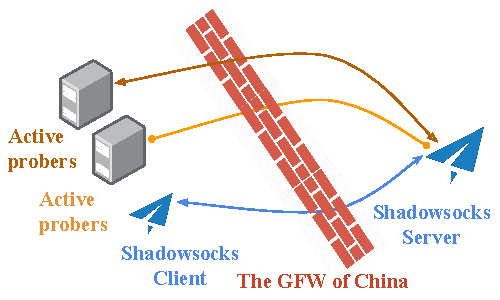
\includegraphics{figures/active_probing.pdf}
\caption{
How active probing works.
A genuine Shadowsocks client connects to a Shadowsocks server;
Once the GFW passively determines that the connection \emph{may} be Shadowsocks,
it directs its active probers to confirm this guess.
}
\label{fig:active-probing}
\end{figure}

Our systematic study
finds that the GFW has started to identify Shadowsocks servers
using a combination of \emph{passive traffic analysis} and \emph{active probing}.
\autoref{fig:active-probing} illustrates the general notion:
the GFW first detects suspected Shadowsocks traffic,
using features like the size and entropy of the first data packet in each connection.
Once a server falls under suspicion,
the GFW sends active probes to it, in different stages,
to confirm whether the server really is Shadowsocks.
The probes are partial replays of past legitimate connections, and random probes of varied lengths.
We suspect that the probes are designed to attack detection vulnerabilities in different implementations of Shadowsocks.
The GFW has been known to use active probing against various circumvention tools
since as long ago as 2011~\cite{Ensafi2015b},
but the techniques now in use against Shadowsocks are new
and more sophisticated than what has previously been reported.

In summary,
our work makes the following contributions:
\begin{itemize}
\item We reveal and systematically study the GFW's latest secret weapon against Shadowsocks.
\item We identify and fingerprint different types of active probes, and infer the probable intention behind them.
\item We derive a more realistic adversary model of replay attacks.
\item We introduce a temporary but effective mitigation against the detection, and provide suggestions for defending against active probing.
\item We have collaborated with the developers of different Shadowsocks implementations to make Shadowsocks more resistant to active-detection attacks.
\end{itemize}

\section{Background on Shadowsocks}
\label{sec:background}

Shadowsocks is an encrypted proxy protocol.
It attempts to avoid detection not by imitating some other protocol,
but by using encryption to appear as a uniformly random byte stream.
There are two components: client and server.
The server is typically installed
on some network outside the censor's control.
The client sends an encrypted target specification to the server.
The server then connects to the target and
begins proxying traffic for the client.
All traffic between the client and the server is encrypted.

It will be important to know a few details of how Shadowsocks encryption works,
in order to appreciate the construction of the probes described in \autoref{sec:probe-types}.
Shadowsocks specifies two main classes
of cryptographic constructions, known in the context of the protocol as
``stream ciphers'' and ``AEAD ciphers''~\cite{spec-shadowsocks}.
The stream cipher construction is cryptographically weak---it
provides only confidentiality, not integrity or authentication,
and for that reason is deprecated.
The AEAD cipher construction (authenticated encryption with associated data)
was developed to fix the flaws of the stream cipher construction,
and provides confidentiality, integrity, and authentication.
Both constructions are keyed by a master password that client and server share,
and both intend to require the client to demonstrate knowledge
of the shared password before using the proxy server
(though as we will see, with stream ciphers the requirement is loose).

With stream ciphers,
the network stream
in both directions is one long ciphertext, preceded by a random initialization vector:
\begin{quote}
\begin{verbatim}
[variable-length IV][encrypted payload...]
\end{verbatim}
\end{quote}
Client and server use the same encryption key,
but different initialization vectors.
The length of the initialization vector may be 8, 12, or 16~bytes,
depending on what cipher is configured.

With AEAD ciphers,
the network stream is a sequence of
length-prefixed chunks, each encrypted and authenticated with an AEAD tag.
To avoid introducing any plaintext for the censor to match on,
the length prefixes are themselves encrypted and tagged.
\begin{quote}
\begin{verbatim}
[variable-length salt]
[2-byte encrypted length][16-byte length tag]
[encrypted payload][16-byte payload tag]
[2-byte encrypted length][16-byte length tag]
[encrypted payload][16-byte payload tag]
...
\end{verbatim}
\end{quote}
The entire stream is preceded by a salt,
which is combined with the shared secret password
to produce a session key for each direction.
The salt may be 16, 24, or 32~bytes.

In both constructions,
the first piece of data the client sends through the tunnel
is a host:port target specification,
whose structure is borrowed from the SOCKS proxy protocol.
The first byte is an address type that indicates the format of the bytes that follow.
The three address types are:
\begin{quote}
\begin{verbatim}
[0x01][4-byte IPv4 address][2-byte port]
[0x03][1-byte length][hostname][2-byte port]
[0x04][16-byte IPv6 address][2-byte port]
\end{verbatim}
\end{quote}

There are many implementations of Shadowsocks~\cite{shadowsocks-libev, outline, shadowsocks-python, shadowsocks-rust, go-shadowsocks2, shadowsocksr-csharp},
and they differ in what features they support.
Not every implementation supports every possible cryptographic construction;
for example,
OutlineVPN~\cite{outline} supports AEAD ciphers only, not stream ciphers.
Some implementations take steps to mitigate replay attacks, and some do not.
This means that a probing adversary may encounter different reactions to probes,
depending on what implementation of Shadowsocks is in use.
In this work,
we focus on two of the more popular implementations,
Shadowsocks-libev~\cite{shadowsocks-libev} and OutlineVPN~\cite{outline},
but the vulnerabilities we describe
may also apply to other implementations.

\begin{table}
    \caption{Timeline of all major experiments. The three set of experiments span weeks and months. Shadowsocks, Sink and Brdgrd refer to the experiments in~\autoref{sec:shadowsocks-server-experiment}, \autoref{sec:conditions-experiments} and \autoref{sec:defense-traffic-analysis} respectively.}
    \label{table:time-span}
    \begin{tabular}{c|c}
      Experiment    & Time span                                 \\ \hline
      Shadowsocks & Sept 29, 2019 -- Jan 21, 2020 (4 months) \\
      Sink & May 16 -- 31, 2020 (2 weeks)    \\
      Brdgrd      & Nov 2 -- 19, 2019 (403 hours)   \\
    \end{tabular}
\end{table}

\subsection{Historical Vulnerabilities and Defenses}
\label{sec:historical-vulns}

In August 2015,
BreakWa11 discovered an active-probing vulnerability in Shadowsocks stream ciphers,
resulting from their lack of integrity protection~\cite{BreakWa112015, Fifield2017-summary}.
An attacker can make many connections to a suspected Shadowsocks server,
and take advantage of ciphertext malleability
to try every possible value of the byte that corresponds to the
address type in the target specification.
Because only 0x01, 0x03, and 0x04 are valid address types,
a known fraction of connections will time out differently from the rest.
Shadowsocks developers mitigated the vulnerability by
having the server not immediately terminate a connection when
a target specification contains an unknown address type~\cite{madeye-timeout}.

Shadowsocks developers attempted to further mitigate the problem
by introducing a ``one time auth'' mode, in which each chunk of data
would carry its own authenticator.
But a lack of integrity protection in chunk length prefixes
led to another active probing vulnerability~\cite{printempw2017, Fifield2017-summary}.
In February 2017, AEAD ciphers became part of the protocol specification,
fixing this authentication problem.

In February 2020, Zhiniang Peng disclosed a devastating vulnerability in Shadowsocks stream ciphers~\cite{Peng2020Redirect, Fifield2020Redirect}.
Using the Shadowsocks server as a decryption oracle,
an attacker,
without knowledge of the shared master password,
can get full decryption of recorded Shadowsocks connections.

\subsection{Past Blocking of Shadowsocks}
\label{sec:historical-blocking}
Since as early as October 2017,
Internet users in China have reported their Shadowsocks servers being blocked,
by port or IP address~\cite{bbs2017blocking, Programthink-Reports2017, Scott-Reports2017}.
Notable blocking events were reported in October 2017 and January 2018,
at the same time as
two important political congresses in China~\cite{bbs2017blocking}.
After the two congresses,
many users reported their servers got unblocked.
Contrary evidence comes from Wiley et~al.,
who during those times were testing Shadowsocks reachability every day
from locations around the world,
but reported not having seen any evidence of Shadowsocks blocking anywhere~\cite{Wiley-Reports2017}.

The reported large-scale blockings mostly happened during politically sensitive times,
including during the 30th~anniversary of the 1989 Tiananmen Square protests,
the 70th~anniversary of the People's Republic of China,
and the 4th~Plenary Session of the 19th~Central Committee of the Communist Party of China.
The most recent spate of reports began around September~16, 2019~\cite{Fifield2019blocking}.

\section{Characterization of Probes and the Probing Infrastructure}
\label{sec:characterization}

Here we describe the experiments we conducted to collect and understand the GFW's active probes.
Based on a collection of 51,837 active probes observed in a number of experiments, we answer the following questions:

\begin{itemize}
    \item What types of probes are observed, and under what conditions?
    \item Where do the probes come from?
    \item Do the probes have any ``fingerprints'' that reveal information about the underlying probing infrastructure?
    \item How long is the delay between a legitimate connection and the probes that react to it?
\end{itemize}

\subsection{Shadowsocks Server Experiment}
\label{sec:shadowsocks-server-experiment}

We set up our own Shadowsocks servers
and attempted to provoke the GFW into probing them.
To do this, we connected to our servers using Shadowsocks clients,
and sent HTTP and HTTPS traffic through the encrypted proxy tunnel,
using web browsers and curl as automated drivers.
We captured packets at both ends for analysis.
We used unmodified clients and servers in all our experiments,
did not create any special firewall rules,
and did not install any obfuscation plugins.
As summarized in~\autoref{table:time-span},
the experiments were conducted over four~months, from September 29, 2019 to January 21, 2020.

Because we could not know in advance
what features the GFW might use to identify Shadowsocks,
we maximized our coverage by using different Shadowsocks implementations and versions,
and by selecting different encryption algorithms.
The two implementations we used were
Shadowsocks-libev~\cite{shadowsocks-libev} and OutlineVPN~\cite{outline}.

\paragraph{Shadowsocks-libev.}
We installed Shadowsocks-libev clients on five VPSes in a Tencent Cloud Beijing datacenter,
and Shadowsocks-libev servers on five VPSes in a Digital Ocean UK datacenter.
Each client was configured to connect to only one of the servers.
Two pairs of the clients and servers used v3.1.3 of Shadowsocks-libev, and the other three pairs used v3.3.1.
As a control, we set up an additional VPS within the same UK datacenter
and never connected to it,
only capturing all incoming traffic.

We generated client traffic using curl.
Through the Shadowsocks proxy, we constantly fetched one of the websites at a given frequency:
\nolinkurl{https://www.wikipedia.org},
\nolinkurl{http://example.com},
and \nolinkurl{https://gfw.report}.

\paragraph{OutlineVPN}
We installed an OutlineVPN v1.0.7 server in a US university network.
The OutlineVPN client we used was the latest as of October 2019.
The client was in a residential network in China.
Client traffic was provided by an instance of Firefox,
configured to automatically browse a subset of the Alexa top 1~million sites that is censored in China.

\paragraph{Limitations.}
The locations of our vantage points lack some diversity,
making us less likely to observe any potential inconsistencies in the probing system
caused by geolocation.

\subsection{Probe Types}
\label{sec:probe-types}

\begin{figure}
    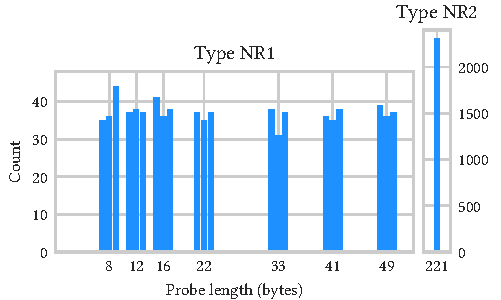
\includegraphics{figures/random-probe-length-distribution}
    \caption{
    Number of occurrences of random probes (type~NR1 and type~NR2) by length.
    Note the two different vertical axes.
    The lengths of type~NR1 probes are evenly distributed in trios
    $(n-1, n, n+1)$ for $n = 8, 12, 16, 22, 33, 41, 49$.
    Type~NR2 probes have length 221 and are roughly three times as common
    % > 2306 / 778.
    % [1] 2.96401
    as all the NR1 probes together.
    }
    \label{fig:random-probe-length-distribution}
\end{figure}

We analyzed all connections to the server port running Shadowsocks,
and used the traffic received by the control host to verify that the probes we observed
were triggered by our own connections,
and not the result of ``background radiation'' Internet scans.
We observed a total of 51,837 active probes across all experiments.
We arrange the probes into two main categories,
replay-based and seemingly random,
with a further distinction of probe types within each category.
The first category of probes, replay-based,
have a payload that is derived from the first data-carrying packet
of some previously recorded legitimate connection.
We assign the probe types in this category names beginning with `R', for ``replay'':
\begin{quote}
\begin{description}
\item[Type~R1] Identical replay.
\item[Type~R2] Replay with byte 0 changed.
\item[Type~R3] Replay with bytes 0--7 and 62--63 changed.
\item[Type~R4] Replay with byte 16 changed.
\item[Type~R5] Replay with bytes 6 and 16 changed.
\end{description}
\end{quote}

Probe types~R3, R4, and~R5 were received only in the OutlineVPN experiment,
not in the Shadowsocks-libev one.
Only two type~R5 probes were received in our experiments.

The other category of probes, seemingly random, have varying lengths.
Their contents that do not resemble a prior legitimate connection in any way we can identify.
We give probe types in this category names starting with `NR', for ``non-replay'':
\begin{quote}
\begin{description}
\item[Type~NR1] Probes of length 7--9, 11--13, 15--17, 21--23, 32--24, 40--42, or 48--50 bytes.
\item[Type~NR2] Probes of length exactly 221 bytes.
\end{description}
\end{quote}

\autoref{fig:random-probe-length-distribution}
illustrates the distribution of type~NR1 and~NR2 probes.
The lengths of NR1 probes are distributed in trios
centered on 8, 12, 16, 22, 33, 41, and 49~bytes.
We will have more to say about this distribution in
\autoref{sec:probe-types-random}.

\subsection{Origin of the Probers}
\label{sec:probe-origin}

\begin{figure}
    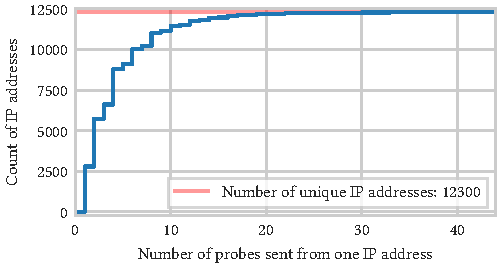
\includegraphics{figures/cdf_ip_occurrences.pdf}
    \caption{
        Cumulative number of probes per prober IP address.
    }
    \label{fig:ip-occurrences}
\end{figure}

A~simple idea to defend against active probing
is to discover the IP addresses of probers, and ban them.
Below, we show it may be challenging to implement such a defense,
because the GFW probes from a large and diverse pool of IP addresses, with high churn.

\paragraph{IP addresses.}
The 51,837 active probes were sent from 12,300 unique source IP addresses,
all located in China.
\autoref{fig:ip-occurrences} shows the distribution of the number of probes sent per unique IP address.
In contrast to previous work, which found that ``95\% of the addresses appear only once''~\cite[\S 5.3]{Ensafi2015b},
in our tests more than 75\% of addresses sent more than one probe.
The most common prober IP addresses are summarized~\autoref{table:source-addr-distribution}.

\begin{table}
\caption{
  The most common prober IP addresses and their number of occurrences.
}
\label{table:source-addr-distribution}
\center
\begin{tabular}{rr}
Prober IP address & Count \\
\midrule
175.42.1.21 & 44 \\
223.166.74.207 & 38 \\
124.235.138.113 & 36 \\
113.128.105.20 & 36 \\
221.213.75.88 & 33 \\
112.80.138.231 & 32 \\
116.252.2.39 & 32 \\
124.235.138.231 & 32 \\
221.213.75.126 & 32 \\
223.166.74.110 & 31
\end{tabular}
\end{table}

We compared our list of prober IP addresses against
934 that were observed to send active probes to Tor servers in 2018 by Dunna et~al.~\cite{Dunna2018a},
and 22,000 that were observed to send various types of active probes between 2010 and 2015 by Ensafi et~al.~\cite{Ensafi2015b}.
\autoref{fig:ip-comparison} shows that three sets overlap only slightly.
We note the IP address 202.108.181.70,
which was responsible for an inordinate number of probes in previous work~\cite[\S 5.3]{Ensafi2015b},
does not appear in our data.
The small overlap is not unexpected, given that past work has observed high churn in prober IP addresses.

\begin{figure}
    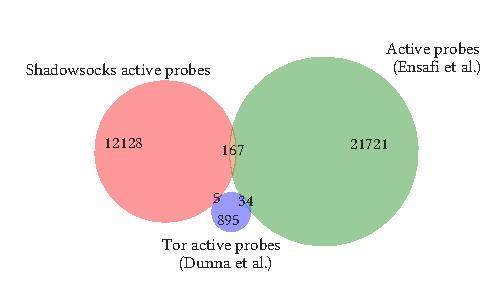
\includegraphics[width=\columnwidth]{./figures/comparison_with_other_probe_source_datasets.pdf}
    \caption{
        Overlap in prober source IP addresses across independently collected datasets.
    }
    \label{fig:ip-comparison}
\end{figure}

\paragraph{Autonomous systems.}

\begin{table}
    \caption{
    Counts of unique prober IP addresses per autonomous system, across all experiments.
    }
    \label{tab:origin-asn}
\begin{tabular}{lr@{\qquad}lr}
AS4837  & 6262 & AS58563 &   44 \\
AS4134  & 5188 & AS17638 &   17 \\
AS17622 &  315 & AS9808  &    2 \\
AS17621 &  263 & AS4812  &    1 \\
AS17816 &  104 & AS24400 &    1 \\
AS4847  &  101 & AS56046 &    1 \\
        &      & AS56047 &    1
\end{tabular}

\end{table}

The autonomous system (AS) distribution of probers is shown in \autoref{tab:origin-asn}.
The two ASes that account for the most Shadowsocks probes are
AS4837 (CHINA169-BACKBONE CNCGROUP China169 Backbone) and AS4134 (CHINANET-BACK\-BONE No.31, Jin-rong Street).
These two were the most common in previous work~\cite{Ensafi2015b, Winter2012a}
as well.
Other ASes that overlap with previous work are
AS17816, AS9808, AS56046, AS17638, AS56047, and AS17622.
AS17622 (CNCGROUP-GZ China Unicom Guangzhou network)
accounts for a much larger fraction of probes than in previous work~\cite[Figure~7]{Ensafi2015b}.
Other previously attested ASes do not appear in our data,
including AS7497 (CSTNET-AS-AP Computer Network Information Center),
which was the third most common source of probes seen by Ensafi et~al~\cite{Ensafi2015b}.
There are also ASes in our dataset
that have not been previously documented as being a source of active probes.

\subsection{Fingerprinting the Probes}
\label{sec:fingerprinting}

As in previous work, we fingerprint the packet-level features
of active probes.
At the IP layer, we examine the ID and TTL fields.
At the TCP layer, we look at source ports and timestamps.

\paragraph{IP~ID and TTL}
We fingerprint the IP~ID and TTL of PSH/\hspace{0pt}ACK packets sent by the probers.
% TODO: add IP ID and IP TTL figure
As in Ensafi et~al.~\cite[\S 5.5]{Ensafi2015b},
we find no clear pattern in the IP~ID sequences,
and that TTLs remain within the range 46--50.

\paragraph{TCP source ports.}

\begin{figure}
    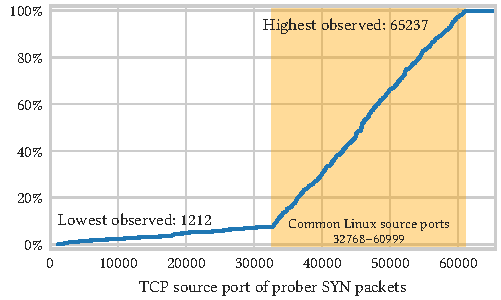
\includegraphics{figures/cdf_source_port_lon15.pdf}
    \caption{
    CDF of TCP source port numbers of probes in one experiment, including 1,576 probes.
    }
    \label{fig:source-ports}
\end{figure}

Around 90\% of probes came from source ports in the range 32768--60999.
This range, highlighted in \autoref{fig:source-ports},
happens to be the default source port range of many Linux kernels.
% Note that the effective range is accessible via the /proc file system at node /proc/sys/net/ipv4/ip_local_port_range.
Probes never used a source port below 1024 (the precise minimum we saw in one experiment was 1212).
These result differ from those of previous work~\cite[\S 5.5]{Ensafi2015b},
which observed all ports being used, and no range of ports being more common than any other.

% Background on TCP timestamps (TSval)
% https://tools.ietf.org/html/rfc7323 section-3
% TSval is just a counter that increases at a fixed rate (e.g. 250 Hz). It gets sent attached to every TCP packet in a special TCP timestamp option. The peer that receives a TCP timestamp option echoes back the received TSval in the TSecr field. The purpose of TCP timestamps is to allow for accurate estimation of round-trip time: when you receive a TSecr, you subtract it from your own current TSval, and divide by the increment frequency, and that's the RTT.
% Often, the TSval counter is initialized to 0 when a machine is rebooted (this is the case with Linux, I believe). One side effect of this fact is that you can estimate a machine's uptime (until it wraps) by seeing a TSval and dividing by the update frequency. (This is what Nmap's uptime guess means.) Other operating systems, for example macOS, initialize the TSval to a random value at boot, so it's not useful for estimating uptime. But the key observation is that the TSval counter is consistent for a single host, and distinct hosts will have distinct sequences (unless they were rebooted at the same time).

% The timer interrupt rate background
% Defined by a compile-time constant called HZ.
% Different platforms use different values for HZ.
% Linux kernel changed HZ for i386 to 250 since 2.6.13.
% The intercept of each line may be used to infer the physical systems uptime. To be more accurate, assuming the TSval counter is initialized to 0 after reboot (which is often the case for Linux), the intercept would be the physical systems uptime moduled by 2 to the 32. The modular operation covers the case where the TSval wraps up, which is indeed observed by us in the figure.

\paragraph{TCP timestamp (TSval).}

\begin{figure}
    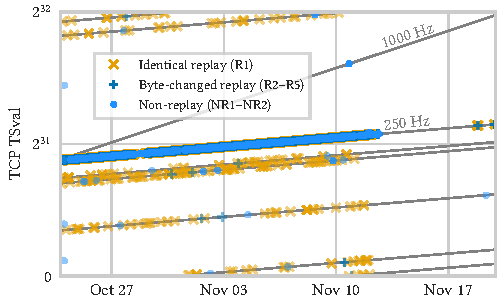
\includegraphics{figures/tsval_lon8.pdf}

    \caption{
    Non-independent processes revealed by
    common TCP timestamp sequences.
    The labeled marker lines have slopes of precisely 250~Hz and 1000~Hz.
    The small cluster of 22~non-replay probes on the 1000~Hz line
    locally have a slope of 1009~Hz,
    but here the measurement is less certain because they span only about~3.5~s.
    The 1000~Hz line does not become 250~Hz, even if connected to one of the sparse non-replay data points at the left edge of the figure.
    }
    \label{fig:tsval}
\end{figure}

The TCP timestamp
is a 32-bit counter that increases at a fixed rate,
attached to every non-RST TCP segment~\cite[\S 3]{rfc7323}.
It is not an absolute timestamp,
but is relative to how and when the counter was initialized,
and its rate of increase varies across operating systems.
\autoref{fig:tsval} shows the timestamp value attached to the SYN segment of each probe.
The figure shows that although the probers use thousands of source IP addresses,
they cannot be fully independent,
because they share a small number of TCP timestamp sequences.
In this case, there are at least seven different physical systems or processes,
with one of the seven accounting for the great majority of probes.
We say ``at least'' seven because we would not be able to distinguish
two processes whose TSvals sequences are very close
(which could happen, for example, if both processes were restarted at about the same time).
We measured the slope of the linear sequences
to be almost exactly 250~Hz,
with the exception of one small cluster of~22 closely spaced points
whose slope is closer to 1000~Hz.
There are two cases where a sequence reached the maximum value of
$2^{32}-1$ and wrapped around to~$0$.
Compare \autoref{fig:tsval} to Figure~11(c) of
Ensafi et~al.~\cite{Ensafi2015b},
which also shows 250~Hz and 1000~Hz sequences.

% TODO: TCP options using the purf?
% ngerprint on TCP options https://ensa.fi/active-probing/imc2015.pdf

\subsection{Delay of Replay Attacks}
\label{sec:delay-of-replay}

The GFW may record the first data-carrying packet of a genuine client connection
and replay it later, possibly with modifications, as an active probe.
\autoref{fig:replay-delay} shows the variability in delay between
when a legitimate connection is made and when the GFW sends replay-based probes derived from that connection.
Because probe payloads may be replayed more than once
(up to 47~times, in one case),
we present two distributions,
with and without repeated payloads.
The orange line represents the delay of the \emph{first} occurrence
of each replay-based probe payload,
while the blue line shows the delay of \emph{all} replay-based probes,
including repeated payloads.
The total number of probes is 3,269 for first occurrences and 11,137 for all occurrences.

More than 20\% of first replays arrived within one second;
more than 50\% within one minute;
and more than 75\% within 15~minutes.
Replay-based probes may be sent almost immediately, or
may be stored for a surprisingly long time before being sent.
The shortest delay we observed was 0.28~seconds
and the longest was 570~hours.

\begin{figure}
    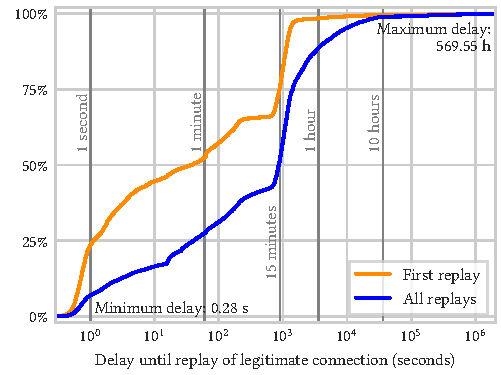
\includegraphics{figures/delay_of_replays_in_all_experiments.pdf}
    \caption{
    CDF of the delay of replay-based probes.
    Note the logarithmic $x$-axis.
    }
    \label{fig:replay-delay}
\end{figure}

\section{What Triggers Active Probing}
\label{sec:conditions}

There are alternative hypotheses for how the GFW might go about discovering Shadowsocks servers.
One is large-scale, \emph{proactive} port scanning;
another is \emph{reactive} probing triggered by legitimate connections.
The fact that the unused control host in \hyperref[sec:characterization]{the previous section}
did not receive any active probes leads us to discard the proactive scanning hypothesis.
Instead, we assume that probes are sent only when the probing system
sees a suspected Shadowsocks connection.

What, then, constitutes a suspected Shadowsocks connection, from the GFW's point of view?
In this section, we deal with the following questions:

\begin{itemize}
    \item How much traffic is required to trigger active probes?
    \item Why were type~R3, type~R4 and type~R5 probes sent only to the OutlineVPN server, not the Shadowsocks-libev server?
    \item Does the GFW consider the length of packets?
    \item Does the GFW consider the entropy of packet payloads?
    \item Do outside-to-inside connections (with the client outside China and the server inside) result in as much active probing as inside-to-outside connections?
\end{itemize}

\subsection{Experiments}
\label{sec:conditions-experiments}

A~convincing way to show what features the GFW uses for traffic analysis is to outline a minimal,
reproducible set of conditions that trigger active probing.
Accomplishing this is, unsurprisingly, the most challenging part of this work,
as it requires us to isolate a small number of features that the GFW really uses,
from countless possibilities.

We are aided by two observations.
First, the byte streams sent between Shadowsocks clients and servers are,
by design, indistinguishable from random.
This means that it may not be necessary to use a real client Shadowsocks implementation;
we may be able trigger active probes by sending random data.
Second, as described in \autoref{sec:delay-of-replay},
replay probes may be sent as soon as 0.28~seconds after a legitimate data packet.
The GFW could have seen only the very beginning
of a client-to-server flow,
before deciding that the traffic was suspicious.

Guided by these two observations,
we implemented a TCP client that connects to a TCP server
and sends one data packet, with a specified length and Shannon entropy.
We implemented a server with two operating modes:
sink mode and responding mode.
In sink mode,
the server accepts TCP connections, but does not respond with any data, and closes connections after 30~seconds.
In responding mode,
the server responds to probers---but not our own clients---with
between 1~and 1000~bytes of random data.

\begin{table}
    \caption{
        Summary of random-data experiments.
        $[x, y]$ means the value is uniformly and randomly sampled from a range, independently for each connection.
        In Exp~1, the server was switched from sink mode to responding mode after 310 hours;
        we label the two subexperiments 1.a and~1.b.
    }
    \label{table:exp-summary}
    \begin{tabular}{c|cc|c}
                              & \multicolumn{2}{c|}{Client} & Server     \\
        Exp~\#                & Length (bytes) & Entropy    & Mode       \\ \hline
        1.a                   & $[1, 1000]$    & $>7$       & sink       \\ \hline
        1.b                   & $[1, 1000]$    & $>7$       & responding \\ \hline
        2\phantom{.a}         & $[1, 1000]$    & $<2$       & sink       \\ \hline
        3\phantom{.a}         & $[1, 2000]$    & $[0,8]$    & sink       \\ \hline
    \end{tabular}
\end{table}

\autoref{table:exp-summary} summarizes the design of the random-data experiments.
\autoref{table:time-span} shows the time span of the experiment.
Clients ran on different VPSes within the same Tencent datacenter in Beijing.
All servers ran in the same Digital Ocean datacenter in the~US.
Client and server IP addresses were not reused across experiments.

\subsection{Experiment Results and Analysis}
\label{sec:traffic-analysis-result}

\paragraph{Little traffic is required to trigger active probes.}
Our sink server, despite not being a real Shadowsocks server
and never sending data,
received many of the same types of probes
as in the Shadowsocks server experiment of \autoref{sec:shadowsocks-server-experiment}.
After a TCP handshake, a single data packet from client to server suffices to trigger active probes.

\begin{figure}
    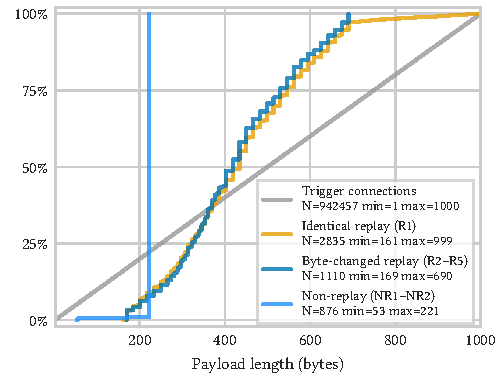
\includegraphics{figures/cdf_payload_length_exp1a.pdf}
    \caption{
      CDF of the payload lengths of replay-based probes over
      the 310~hours of Exp~1.a.
      The lengths of replay probes exhibit a stair-step pattern.}
    \label{fig:replay-payload-length}
\end{figure}

%% The analysis below is based on the following output:
%% [168,264): total: 376; remainder 9: 273(72.6%);
%% [264,384): total: 749; remainder 9: 276(36.8%); remainder 2: 243(32.4%);
%% [384,688): total: 1558; remainder 2: 1494(95.9%);
%% One can generate these output with:
%% cd figures && make cdf_payload_length_exp1a.pdf
\paragraph{Only certain lengths are replayed.}
Although our clients sent data packets with lengths of between 1~and 2000~bytes,
virtually all probes that were determined to be replays had a payload length of between 160~and 700~bytes,
with the maximum length being 999 bytes.
\autoref{fig:replay-payload-length} shows the distribution of probe lengths in Exp~1.a.
The distribution of lengths exhibits a stair-step pattern,
reflecting the fact that certain lengths are more likely to be replayed.
Namely, the lengths of replay probes tend to have certain remainders when divided by~16.
Considering type~R1 probes (type~R2 is similar),
of the 376 probes whose length is in the interval 168--263 bytes,
72\%~have a length whose remainder when divided by~16 is~9;
of 1,558 in the interval 384--687,
96\%~have a length whose remainder is~2;
and of 749 in the middle interval 264--383,
there is a mix of remainders 9~(37\%) and 2~(32\%).
The results suggest that the GFW considers packet lengths in classifying Shadowsocks traffic.
Packet length is a reasonable feature to use,
because Shadowsocks does not pad the contents of the tunnel,
only incidentally changing the underlying packet length distribution by adding
an address header prefix (see \autoref{sec:background}) and,
with AEAD ciphers, length prefixes and tags.
The payload length distribution of the Shadowsocks traffic therefore resembles
that of the underlying traffic, which is often HTTP or~TLS.

\begin{figure}
    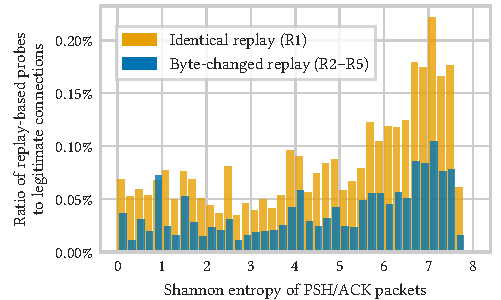
\includegraphics{figures/replayed_ratio_exp3.pdf}
    \caption{
    Rate of replay-based probes per legitimate connection in Exp~3,
    according to per-byte entropy of the legitimate connection.
    }
    \label{fig:replay-payload-entropy}
\end{figure}

\paragraph{High-entropy packets are more likely to be replayed.}
Two pieces of evidence support this conclusion.
First,
\autoref{fig:replay-payload-entropy} shows that
while packets of all entropies may be replayed,
one with a high per-byte entropy of~7.2 is almost four times as likely
to be replayed as one with a low entropy of~3.0.
Second,
Exp~1.a and Exp~2 differ only in the entropy of packets,
and over the same period of time,
the server in Exp~1.a received significantly more probes than the one in Exp~2.

\paragraph{Probes of type~R3 and~R4 are not sent unless the server has previously responded to probes of type~R1 and~R2.}
The thousands of probes received in Exp~1.a, Exp~2, and Exp~3
could all be classified as type~R1, R2, or~NR2.
In other words,
we were not able to trigger probes of types~R3, R4, R5 or NR1 in these experiments.
This result reminded us of the fact that in the experiment of \autoref{sec:shadowsocks-server-experiment},
type~R3, R4 and~R5 probes
were only ever received by OutlineVPN servers,
and not by Shadowsocks-libev servers.

As will be expanded on in \autoref{sec:probe-types-replay},
one major difference between Shadowsocks-libev and the version of OutlineVPN we used
is that Shadowsocks-libev has a filter to defend against replay attacks,
and OutlineVPN does not.
(At least in the version we used---OutlineVPN has since added replay protection~\cite{outline-v1.1.0}.)
For this reason,
Shadowsocks-libev servers does not respond to exact replays of earlier connections,
while OutlineVPN servers do.

We therefore hypothesize that the GFW does not send probes of type~R3, R4, and~R5
unless the server has already responded to probes of type~R1 and~R2.
We switched the server in Exp 1.a to responding mode after 310 hours of operating in sink mode.
Soon after the server started responding to type~R1 and type~R2 probes,
it began to receive a large number of type~R3 and type~R4 probes.
The server continued to receive type~R1 and~R2 probes as well.

These results suggest that the active probing system operates in stages.
It does not move on to the next stage until a certain condition is observed.
This implementation detail suggests that the censor may have designed its
active probing system with not only Shadowsocks in mind.
Other, similarly behaving protocols may also be targeted.

We do not know why type~R5 and type~NR1 probes did not appear in any of our four random-data experiments.


\paragraph{New probe types observed.}

The sink/responding servers received probes that did not match
the probe types seen in our earlier experiment with Shadowsocks-libev and OutlineVPN.
In Exp~1.b, we saw 11 replay-based probes that had bytes from 16 to 32 changed.
We additionally saw many non-replay probes across all four experiments.
In total, there were
9~probes of 53~bytes,
5~probes of 56~bytes,
3~probes of 169~bytes,
1~probe of 180~bytes, and
1~probe of 402~bytes.

\paragraph{The GFW does not distinguish traffic directionality.}
We set up a Shadowsocks server inside China and made connections to it from outside.
The traffic proxied was generated by automatically browsing a subset of Alexa top 1 million websites.
The server received a large amount of active probing.
This result indicates that the GFW probes suspected servers
regardless of whether the server is inside or outside China.
This bidirectional triggering behavior differs from Winter and Lindskog's~\cite[\S 4.4]{Winter2012a} observation
that outside-to-inside Tor connections did not trigger active probing.
On the other hand,
the GFW is known not to distinguish traffic directionality for many protocols,
including DNS~\cite[\S 2]{Anonymous2014a}, HTTP~\cite[\S 3]{Clayton2006a} and TLS~\cite[\S 3.1]{Chai2019a}.
The GFW's sensitivity to directionality has even been known to change over time,
as in the case of TLS ESNI blocking, which was bidirectional for two weeks
before becoming unidirectional~\cite{Bock2020ESNI}.

% commented out, because this can be misinterpreted,
% we do not have any SS-libev servers blocked anyway.
% Despite being probed, our China-based server was not blocked throughout the experiment.

\section{Intention Behind the Probes}
\label{sec:intention}

As discussed in \autoref{sec:probe-types},
we discovered seven distinct types of active probes to our Shadowsocks servers.
A~natural question is: what information can the GFW get from these probes?
Unlike in previous work~\cite{Ensafi2015b, Winter2012a},
for us this question cannot be answered by a simple glance at the probes.
We conjecture that if the probes elicit reactions from a Shadowsocks server
that differ from the reactions of non-Shadowsocks servers,
the GFW can be confident in classifying the server as Shadowsocks.

Therefore, understanding the effects of those probes on Shadowsocks servers is key.
We developed our own prober simulator
to observe how Shadowsocks servers react to probes like those sent by the GFW.
We further checked the source code of Shadowsocks implementations to understand their internal logic.
Based on this analysis,
we formed conjectures regarding what distinguishable server reactions
may be exploited for classification.

\subsection{Prober Simulator Experiment}
\label{sec:intention-simulator}

We developed a prober simulator that can send all seven types of probes to Shadowsocks servers, and record their reactions.
The prober simulator allows us to test a wide range of Shadowsocks implementations,
with different configurations, efficiently and locally.
In addition, the prober simulator lets us cover implementation corner cases
and reveal some fingerprintable features that may have not been exploited by the GFW.

\paragraph{Replay-based probes.}
To simulate replay-based probes,
the simulator records the first data-carrying packet in a connection between a Shadowsocks client and server,
then sends the data to the server in a separate connection.
To send byte-changed probes,
the simulator randomly changes certain bytes of the payload to different values.

\paragraph{Non-replay probes.}
To simulate non-replay probes,
the simulator simply sends a specific number of random bytes.
The justification here is that the servers' reactions to
the GFW's non-replay probes are no different from their reaction to random probes.
For comprehensiveness,
we let the simulator send random probes with lengths of between~1 and 99~bytes,
as well as probes of 221~bytes.

% For each Shadowsocks implementation,
% simulator automatically configures and starts its server and send the probes to its listening port.
% The simulator will also capture traffic, record server reactions and keep server logs for later analysis.

% -3.3.3: Archlinux, Debian Stretch-backport-sloppy, CentOS 7, 8 (outman), Fedora 30, 31 (outman), openSUSE Leap 15.1
% -3.2.5: Ubuntu 19.04, Deban Buster, stretch-backport
% -3.2.0: Recent Fedora versions (until EOL) / RHEL 6, 7 and derivatives (including CentOS, Scientific Linux) EPEL 6-7, Fedora 27-31 (librehat
% )
% -3.3.1: Ubuntu 19.10, docker in our experiments, ss (modified) in our experiments
% -3.1.3: Ubuntu 18.04 LTS
% -2.6.3: Debian Stretch

%\textbf{Tested clients.}

\begin{figure*}
    \begin{subfigure}[b]{\textwidth}
    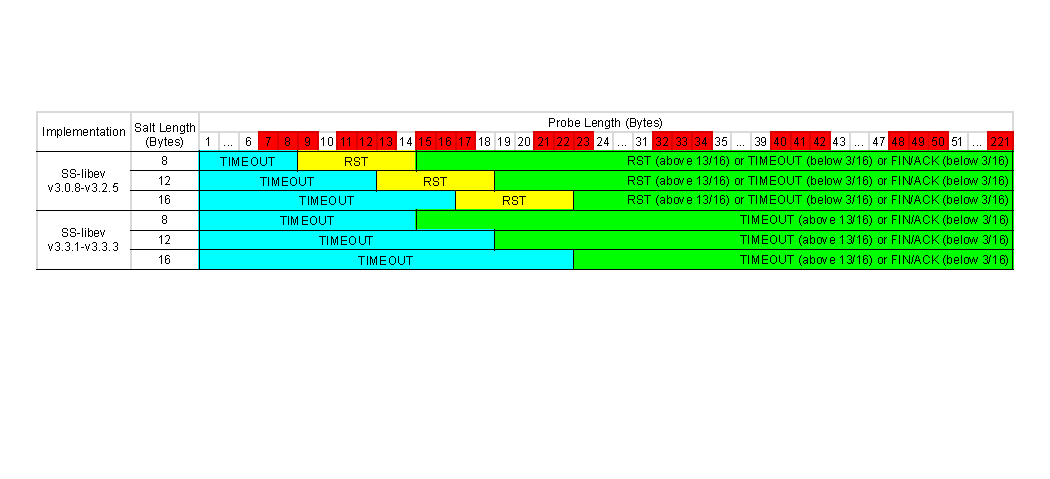
\includegraphics[trim={0cm 3.5cm 0cm 1.9cm},clip]{./figures/reaction_to_random_probes_stream_cipher.pdf}
    \caption{Stream ciphers}
    \label{fig:random-probes-reactions:stream}
    \end{subfigure}

    \begin{subfigure}[b]{\textwidth}
    %%  trim={<left> <lower> <right> <upper>}
    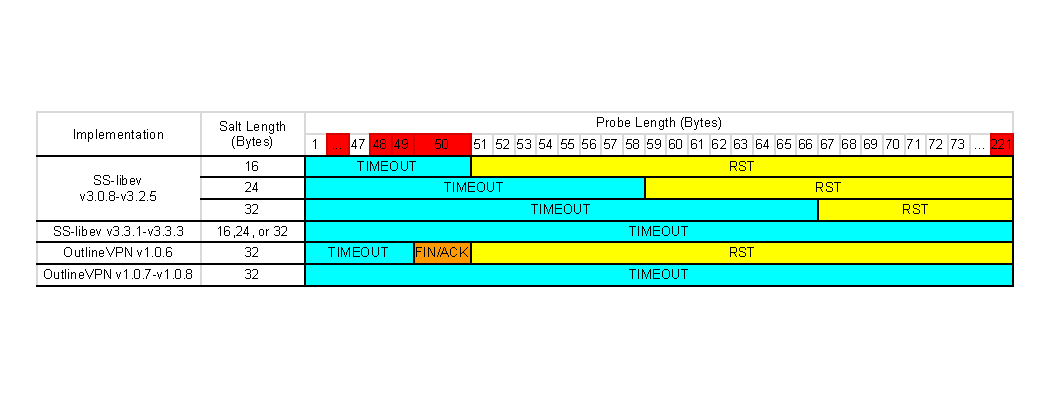
\includegraphics[trim={0cm 2.2cm 0cm 1.8cm},clip,width=\columnwidth]{./figures/reaction_to_random_probes_aead_cipher.pdf}
    \caption{AEAD ciphers}
    \label{fig:random-probes-reactions:aead}
    \end{subfigure}

    \caption{
    Reactions of Shadowsocks servers to synthetic random probes with different lengths.
    \autoref{fig:random-probes-reactions:stream} is for servers using the stream ciphers construction and
    \autoref{fig:random-probes-reactions:aead} is for the AEAD ciphers construction.
    Payload lengths that the GFW has been observed to send are marked in red.
    ``TIMEOUT'' means the server waits until the prober or itself times out.
    ``RST'' means the server sends an immediate TCP RST.
    ``FIN/ACK'' means the server will be the first to send a FIN/ACK to close the connection.
    }
    \label{fig:random-probes-reactions}
\end{figure*}


\paragraph{Choice of servers.}
We chose a set of Shadowsocks implementations that has significant coverage over the Shadowsocks circumvention ecosystem.
Specifically,
we tested the Shadowsocks implementations that met any of the following conditions:
1)~is available in a repository of a major Linux distribution;
2)~is available in the pip repository;
3)~is the latest version;
4)~is widely used by any popular one-click script;
5)~has a recent fix to any distinguishable reactions as the result of a preliminary report on these attacks; or
6)~was recommended to us by developers.
Using this selection process,
we chose Shadowsocks-libev (v3.0.8, v3.1.3, v3.2.5, v3.3.1, and v3.3.3) and OutlineVPN (v1.0.6, v1.0.7, and v1.0.8).

\subsection{Intention Behind Random Probes}
\label{sec:probe-types-random}

\subsubsection{Servers' reactions to random probes}

\autoref{fig:random-probes-reactions} summarizes the reactions of different Shadowsocks implementations
to random probes of various lengths.
For each implementation,
we group their available encryption methods
first by stream ciphers versus AEAD ciphers,
then by the size of their initialization vector (IV) or salt.
For example, among the stream ciphers supported by Shadowsocks-libev are
``aes-128-ctr'' and ``aes-256-cfb''.
Both of these have a 16-byte IV,
so we group them in the ``16~bytes'' row.
Refer to \autoref{sec:background} for the meaning of IV and salt in the context of Shadowsocks protocols.

Server reactions in \autoref{fig:random-probes-reactions} are represented by the codes ``TIMEOUT'', ``RST'', and ``FIN/ACK''.
TIMEOUT means that the server waits for more data, until either it or the prober reaches a timeout.
The GFW usually times out in less than 10~seconds,
while the default timeout value for many Shadowsocks implementations is 60~seconds.
Therefore, TIMEOUT typically means that the prober, and not the server,
is the first to send a FIN/ACK to close the connection.
FIN/ACK and RST mean that the server sends either a FIN/ACK or a RST immediately.
The choice of FIN/ACK or RST may depend on OS-level socket handling.
Frolov et~al.\ showed~\cite[\S IV.C]{Frolov2020a}
that when closing a socket on Linux,
a FIN/ACK will be sent if the application has read all the data from its kernel socket buffer;
otherwise a RST will be sent.

\autoref{fig:random-probes-reactions} demonstrates that different implementations using different forms of encryption
have fingerprintable reactions to probes of varying lengths.
Below we discuss how the GFW may exploit these reactions
in each Shadowsocks implementation.

\paragraph{Shadowsocks-libev v3.0.8--v3.2.5 with stream ciphers.}
Take the first row in \autoref{fig:random-probes-reactions:stream}
as an example.
Shadowsocks-libev v3.0.8--v3.2.5 servers with an 8-byte IV
exhibit three reactions, depending on the length of the random probe.
When the length of a probe is 1--8 bytes,
the server always times out.
This is because the server has only received a (partial) IV
and is awaiting a target specification.

When the length of a probe is 9--14 bytes,
the server usually sends an immediate RST,
because it has not received a complete target specification.
The shortest random probe likely to decrypt to a meaningful specification is 15~bytes,
which meets the minimal length requirement of a complete IPv4 specification (see \autoref{sec:background}).
A~hostname specification could be slightly shorter than 15~bytes,
but only if the 1-byte hostname length field happens to decrypt to the value~1 or~2.

When the length of a probe is 15 or more bytes,
the server may have any of the three possible reactions:
RST, TIMEOUT or FIN/ACK.
The reaction depends on whether the random payload decrypts to a meaningful target specification.
The first requirement for a meaningful target specification is that the
address type must be one of the values 0x01, 0x03, or 0x04;
any other value results in an immediate RST.
Because the address type is a 1-byte field, we might expect
to see an immediate RST in a $1 - \frac{3}{256}$ fraction of tests.
What we actually see is a fraction closer to $1 - \frac{3}{16}$.
The reason for this is that Shadowsocks-libev masks out the upper 4~bits of the field
(an artifact of the ``one time auth'' scheme mentioned in \autoref{sec:historical-vulns}).
% TODO: show the plot if have enough space.
The probability of a RST reaction decreases with longer probes,
because longer probes are more likely to contain a complete IPv6 address specification,
or a hostname length that is consistent with the packet length.

Upon receiving a complete target specification,
the Shadowsocks server tries to connect to the given target.
Specifically, when the address type field decrypts to 0x04,
the server tries to resolve the hostname;
when the address type is 0x01 or 0x03,
the server sends a SYN packet to the target's IP address and port.
Since this behavior is a connection to an essentially random IP address or hostname,
the connections almost always fail;
and when that happens,
the server sends a FIN/ACK to the client to close the connection.
If the remote connection does not fail immediately
(for instance, if the remote host does not respond and the Shadowsocks server
spends time retransmitting SYN packets),
the GFW's probers will be the first to close the connection with a FIN/ACK.

\paragraph{Shadowsocks-libev v3.0.8--v3.2.5 with AEAD ciphers.}
With AEAD ciphers, servers have a different set of fingerprintable reactions.
The first row in \autoref{fig:random-probes-reactions:aead} represents
an AEAD cipher with a 16-byte salt.
When the probe length is less than or equal to 50~bytes,
the server times out waiting for more data.
It wants there to be at least enough data for the salt (16~bytes),
encrypted length prefix (2~bytes),
encrypted length tag (16~bytes),
and another tag (16~bytes) for the first encrypted data payload.
% https://github.com/shadowsocks/shadowsocks-libev/blob/64d3235c67f235aea35133f601fa1b521adbf8dc/src/aead.c#L589-L590
Once 51~bytes or more are received,
the server tries to decrypt the data received,
which invariably fails with an authentication error.
(Unlike with stream ciphers, where random data may by chance decrypt to something meaningful,
with AEAD ciphers, the probability of that happening is negligible.)
The server sends out an immediate RST because of the authentication error.

\paragraph{Changes in Shadowsocks-libev v3.3.1--v3.3.3.}
The parsing logic for Shadowsocks-libev v3.3.1--v3.3.3 is very similar to what we just described above for Shadowsocks-libev v3.0.8--v3.2.5.
The only difference, as shown in \autoref{fig:random-probes-reactions:aead},
is that the server always times out instead of sometimes sending an immediate RST~\cite{ss-libev-timeout}.

\paragraph{OutlineVPN v1.0.6.}
OutlineVPN exclusively uses the AEAD cipher construction of Shadowsocks,
and only with the ``chacha20-ietf-poly1305'' method, which has a 32-byte salt.
In OutlineVPN v1.0.6,
when the probe length is less than 50~bytes, the server times out.
The server wants 50~bytes in order to parse the following structure:
\begin{quote}
\begin{verbatim}
[32-byte salt]
[2-byte encrypted length][16-byte length tag]
\end{verbatim}
\end{quote}
Unlike Shadowsocks-libev,
the OutlineVPN server does not additionally wait for enough data
for there to be a second tag.
More uniquely, the OutlineVPN server sends a FIN/ACK immediately
when it receives a probe of exactly 50~bytes.
When the probe length is greater than 50~bytes, the server sends an immediate RST due to an authentication failure.

\paragraph{OutlineVPN v1.0.7--v1.0.8.}

Starting in OutlineVPN v1.0.7,
the developers fixed the server's distinguishable reactions~\cite{outline-timeout, Frolov2020a}.
Like the newer versions of Shadowsocks-libev using AEAD ciphers,
the server always times out,
regardless of probe length.

\subsubsection{How an attacker might use the information from random probes}

We use the general term ``attacker'' instead of ``GFW''
in this section for two reasons.
First, attacks may be performed not only by the GFW,
but by any censor capable of observing Shadowsocks traffic.
Second, due to the black-box nature of the GFW,
we can only guess at its internal logic and cannot confirm our suspicions.

An attacker can identify a Shadowsocks server with high confidence
using statistical analysis of its reactions to random probes.
Specifically, an attacker can send a set of probes with varying lengths to the server and record its reactions.
After collecting enough reactions,
the attacker may perform a statistical analysis.
A~server whose reactions fit into one row of \autoref{fig:random-probes-reactions}
is then very likely to be a Shadowsocks server.
The fact that the GFW needs only a single probe to detect and block a Tor server~\cite{Winter2012a},
but a set of several probes before blocking a Shadowsocks server,
suggests that the GFW does some statistical analysis of this kind to detect Shadowsocks.

The attacker may even be able to infer the length of the IV
in older Shadowsocks implementations.
Furthermore, when the IV is inferred to be 12~bytes long,
the attacker knows that the cipher used is ``chacha20-ietf'',
because that is the only supported cipher with a 12-byte IV~\cite[\S~Stream~Cipher]{spec-shadowsocks}.

By similar reasoning,
an attacker may be able to infer which Shadowsocks implementation is in use,
and its approximate version.
For example, whether an authentication error results in a RST or a TIMEOUT
can be used to determine if the server is running an older or newer implementation~\cite{Frolov2020a}.
Whether the probability of RST is around $1 - \frac{3}{256}$ or $1 - \frac{3}{16}$
determines whether the Shadowsocks implementation applies a mask to the address type field.

In practice, the GFW is observed to send a set of type~NR1 and NR2 probes to the same server.
Instead of sending the probes all at once,
the GFW sends a few of them in each hour.
We conjecture that the GFW does this in order to make the probes less noticeable and harder to fingerprint.
A~design like this also allows the GFW to use resources in a more balanced and efficient way.

The probe lengths that the GFW sends, marked in red in \autoref{fig:random-probes-reactions},
coincide with thresholds at which reactions change in certain Shadowsocks implementations.
For example, a server that uses ciphers with 8-byte IVs will time out 8-byte probes, and immediately RST 9-byte probes.
The GFW covers this transition point by sending probes of length 7, 8, and 9~bytes.
However it is worth noting that
type~NR1 probes of length 32--34 bytes and 40--41 bytes, as well as type~NR2 probes of length 221~bytes,
do not coincide with any server thresholds.
However, they may still be useful to identify Shadowsocks servers.
Depending on implementation,
these probes may be used to calculate the empirical probability for a server to send a RST.
If the possibility is close to $1 - \frac{3}{256}$ or $1 - \frac{3}{16}$,
the attacker may infer that the Shadowsocks server uses stream ciphers.

\subsection{Intention Behind Replay-based Probes}
\label{sec:probe-types-replay}

\paragraph{Servers' reactions to replay-based probes.}

\autoref{table:reactions-to-replay} summarizes various servers' reactions to replay-based probes.
This table only covers the case where replays are long enough to contain a complete target specification,
because,
in the absence of external traffic shaping,
the genuine payloads on which the replays are based
are always long enough to contain that information.

\paragraph{Implementations without a replay defense mechanism.}
The reaction of a server to type~R1 identical replays depends on whether it has a replay defense mechanism or not.
Servers without a replay defense mechanism, such as OutlineVPN v1.0.6--v1.0.8,
respond to identical replay with a stream of data in one or many packets.
As soon as a prober receives data,
it ACKs the data and sends FIN/ACK to close the connection.

An adversary might even guess what protocol is being proxied,
by checking if the length of
the server's responses are always the same for a given replayed payload.
Although the responses of the Shadowsocks servers are encrypted,
a consistent response length may suggest that the underlying message
is an HTTP response or TLS ServerHello, for example.

A~key observation is that the offsets of the bytes that change in probe types~R2, R3 and~R5 contain the IV or salt.
This means that a Shadowsocks server's reactions to these probes are no different from the random probes discussed in \autoref{sec:probe-types-random}.
Type~R4 probes may be a chosen ciphertext attack, targeting Shadowsocks servers that use stream ciphers with a 16-byte IV.
Comparing to probes of type~R2, R3 and~R5,
which are also essentially chosen cipher attacks,
type~R4 is more fine-grained,
because a censor can get the exact probability of each reaction by enumerating all 255 altered byte values.

\paragraph{Implementations with a replay defense mechanism.}

Even with a replay defense mechanism, the behaviors of a Shadowsocks implementation may be distinguishable.
For example, Shadowsocks-libev implements its replay defense using
a Bloom filter that remembers what IVs and salts have already been received~\cite{bloom-filter}.

\begin{table}
    \caption{
    Servers' reactions to identical replays (type~R1) and byte-changed replays (types~R2--R5) differ depending on replay detection and stream/AEAD ciphers.
    R:~Reset, T:~Timeout, F:~FIN/ACK, D:~Sending Data. Here we assume all replays are long enough to contain a complete IV and target specification.
    }
    \label{table:reactions-to-replay}
    \begin{tabular}{cccc}
    Implementations                                                                             & \begin{tabular}[c]{@{}c@{}}Encryption\\ Mode\end{tabular} & \begin{tabular}[c]{@{}c@{}}Identical \\ Replay\end{tabular} & \begin{tabular}[c]{@{}c@{}}Byte-changed\\ Replay\end{tabular} \\ \hline
    \multirow{2}{*}{\begin{tabular}[c]{@{}c@{}}Shadowsocks-libev\\ v3.0.8--v3.2.5\end{tabular}} & Stream                                                    & R\phantom{/T/F/D}                                           & R/T/F                                                         \\ \cline{2-4}
                                                                                                & AEAD                                                      & R\phantom{/T/F/D}                                           & R\phantom{/T/F}                                               \\ \hline
    \multirow{2}{*}{\begin{tabular}[c]{@{}c@{}}Shadowsocks-libev\\ v3.3.1, v3.3.3\end{tabular}} & Stream                                                    & \phantom{R/}T\phantom{/F/D}                                 & \phantom{R/}T/F                                               \\ \cline{2-4}
                                                                                                & AEAD                                                      & \phantom{R/}T\phantom{/F/D}                                 & \phantom{R/}T\phantom{/F}                                     \\ \hline
    OutlineVPN                                                                                  & AEAD                                                      & \phantom{R/T/F/}D                                           & \phantom{R/}T\phantom{/F}                                     \\ \hline
    \end{tabular}
\end{table}

As shown in \autoref{table:reactions-to-replay},
when AEAD ciphers are used,
servers' reactions to identical and byte-changed replays are consistent.
However, when stream ciphers are used,
the servers' reactions to identical and byte-changed replays are inconsistent.
For identical replays,
Shadowsocks-libev v3.0.8--v3.2.5 is guaranteed to send a RST immediately;
while the same server receiving byte-changed replays will have one of three different reactions: Reset, Timeout, or FIN/ACK.

Furthermore, with stream ciphers,
an attacker can detect whether a replay filter exists.
For example, the attacker can send the same random probe to the server twice.
If the first probe happens to cause an outgoing connection to some remote server,
while the second probe is blocked by the replay filter,
the difference in the timing of responses will tell the attacker
that a replay filter is in place.
Although we cannot confirm that this is the exact logic used by the GFW,
we did observe that around 10\% of type~NR2 probes were sent to the same server more than once.

\section{GFW's Blocking Module}
\label{sec:blocking}

% In total, we used 63 vantage points: 26 vantage points in China (2 residential network, 24 Tencent Cloud and Alibaba Cloud); 17 vantage points in UK (Digital Ocean) and 18 (13 Digital Ocean, 4 Amazon AWS and 1 university network), 2 in Netherland (Digital Ocean)
Since July 2019,
we have been running experiments on 63 vantage points in China, the US, the UK, the Netherlands, and Singapore.
Each vantage point was used either as a server or a client.
We used various Shadowsocks implementations~\cite{shadowsocks-libev, outline, shadowsocks-python, shadowsocksr-csharp} and settings.
Interestingly, although many of our VPSes have been under intensive active probing,
only three have been blocked.
In this section,
we analyze and speculate on the nature of the blocking and unblocking mechanism used by the GFW.

% Anecdotal reports if port is changed, then IP blocking.

\paragraph{Block by port, or by IP address?}
The three blocked servers were not all blocked in the same way.
Some were blocked by dropping all traffic from a specific server port (block by port),
and some by dropping traffic from all ports (block by IP address).
In either case, only the server-to-client direction was blocked.
This method of unidirectional packet dropping, or null routing,
is similar to the way GFW blocks Tor servers,
as shown in previous work~\cite{Winter2012a}.

It may be reasonable, from the censor's point of view, to block an entire IP address.
The servers running Shadowsocks are usually dedicated solely to circumvention,
and do not host other services that the censor cares to keep accessible,
so there is little harm to the censor in blocking the server entirely.

\paragraph{When to unblock?}
% TODO: citation needed
GFW is known to probe blocked Tor servers every 12~hours,
and unblock them when Tor no longer appears to be running~\cite{Winter2012a}.
In contrast, in our experiments,
we saw no regular checks to see whether blocked servers were still running Shadowsocks.
One of our servers became unblocked more than a week after being blocked.
The server had continued to run Shadowsocks even after being blocked,
and we observed no probes to the server before the GFW unblocked it.
This may be because,
as explained in \autoref{sec:probe-types-random},
it takes more probes to confirm Shadowsocks than it does Tor,
making post-block checks more expensive.

% TODO: well, the server got blocked is not even Shadowsocks sever, its ShadowsocksR.
% ShadowsocksR server: we confirm, the server port is blocked sometimes before Beijing Time 10/29 2-11 AM.

% The conference is between 2019/10/28 and 2019/10/31, Beijing Time. Until 1572617445.114782000, Beijing Time: Friday, November 1, 2019 10:10:45.114 PM, the port is still blocked, the block is one direction from server to client. Before 1572696923.730123000, Beijing Time: Saturday, November 2, 2019 8:15:23.730 PM, the port is unblocked.

% The precise time can only be narrowed down to this. We did not observe any active probing or any suspicious traffic coming to the Shadowsocks port during the block of the Shadowsocks-server.

% This is interesting, like the GFW does not even bother to check before unblocking a server. Its unblocking is more like a human controlled factor based on timing.

%The server is blocked and unblocked after this political conference in China: https://zh.wikipedia.org/zh/%E4%B8%AD%E5%9B%BD%E5%85%B1%E4%BA%A7%E5%85%9A%E7%AC%AC%E5%8D%81%E4%B9%9D%E5%B1%8A%E4%B8%AD%E5%A4%AE%E5%A7%94%E5%91%98%E4%BC%9A%E7%AC%AC%E5%9B%9B%E6%AC%A1%E5%85%A8%E4%BD%93%E4%BC%9A%E8%AE%AE

% The server is blocked and unblocked after this political conference in China: https://zh.wikipedia.org/zh/%E4%B8%AD%E5%9B%BD%E5%85%B1%E4%BA%A7%E5%85%9A%E7%AC%AC%E5%8D%81%E4%B9%9D%E5%B1%8A%E4%B8%AD%E5%A4%AE%E5%A7%94%E5%91%98%E4%BC%9A%E7%AC%AC%E5%9B%9B%E6%AC%A1%E5%85%A8%E4%BD%93%E4%BC%9A%E8%AE%AE

\paragraph{Why were our servers rarely blocked?}

While the fact that active probing happens is clear,
it is still unclear to us how active probing relates to the blocking of Shadowsocks servers.
Few of the servers that received probes were blocked.
One of the servers that was blocked had operated for only around 15~minutes,
and had not received nearly as many probes as other servers that did not get blocked.

%The small blocking server sample makes any causal hypothesis on the blocking and unblocking of Shadowsocks server harder to falsify.

We have two hypotheses attempting to explain this phenomenon.
One is that the blocking of Shadowsocks is controlled by human factors.
That is, the GFW may maintain a list of detected or suspected Shadowsocks servers,
and it is up to a human decision whether the servers on the list should be blocked or not.
This hypothesis would partially explain why more blocking has been reported during politically sensitive periods of time~\cite{bbs2017blocking, Fifield2019blocking}.

Another hypothesis is that active probing is ineffective against the particular Shadowsocks implementations and versions that we used in most of our experiments.
Indeed, all three servers that got blocked were running ShadowsocksR~\cite{shadowsocksr-csharp} or Shadowsocks-python~\cite{shadowsocks-python},
which differ from the Shadowsocks-libev~\cite{shadowsocks-libev} and OutlineVPN~\cite{outline} implementations we used in most of the experiments.
However, numerous user reports suggest that Shadowsocks-libev and OutlineVPN are not immune to being blocked, in general.

% The third hypothesis is there exists some geolocation inconsistency in censorship.
% All three servers that got blocked were running Amazon AWS servers, different from the Digital Ocean datacenter in all other experiments.
% In addition, they were connected from a different residential network than the ones used in most of the other experiments.
% This hypothesis can be true if the GFW pays special attention to address ranges belonging to certain known data centers,
% or pays special attention to connections from some specific residential networks.

\section{Circumvention}
\label{sec:circumvention}

The detection of Shadowsocks happens in two stages:
1)~passive identification of suspected Shadowsocks connections, then
2)~active probing of the server.
Therefore, to avoid blocking, one can
1)~evade the passive detector, or
2)~respond to active probes in a way that does not result in blocking.
Below, we introduce and discuss these two circumvention strategies.
We have shared our findings and proposed defenses with the developers of Shadowsocks-libev and OutlineVPN,
which has led to improvements to those tools (see~\autoref{sec:responsible-disclosure}).

\subsection{Defense Against Traffic Analysis}
\label{sec:defense-traffic-analysis}

\paragraph{Changing payload lengths in the client-to-server stream is effective.}

In \autoref{sec:traffic-analysis-result},
we showed that the GFW considers the length of the first data packet in a connection to identify Shadowsocks traffic.
This finding suggests that
we can mitigate the GFW's traffic analysis attack
by altering packet lengths.

Brdgrd~\cite{brdgrd} (bridge guard) is software that can be run on a Shadowsocks server that causes the client to break its Shadowsocks handshake into several smaller packets.
Brdgrd was originally intended to disrupt the detection of Tor bridges by forcing the GFW to do complicated TCP reassembly~\cite{Winter2012a},
but here we take advantage of its ability to shape client packet sizes.

As a test, we set up a Shadowsocks server and let a Shadowsocks client make 16~connections to it every 5~minutes.
We enabled and disabled brdgrd at random times,
and measured the rate of active probing under both conditions.
\autoref{table:time-span} summarizes the time span of the experiment.

\begin{figure}
    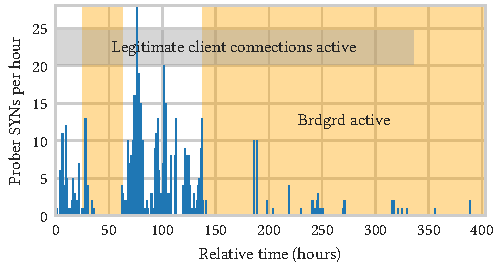
\includegraphics{figures/effectiveness_of_brdgrd.pdf}
\caption{
The intensity of active probing diminishes when brdgrd is active.
}
\label{fig:brdgrd}
\end{figure}

\autoref{fig:brdgrd} shows the number of probes received by the Shadowsocks server over time.
It shows probing going to zero within a few hours of activating brdgrd.
As soon as we disabled brdgrd again, active probing resumed.
The second time we enabled brdgrd,
probing completely stopped for around 40~hours, but later a few more probes arrived.
Note that receiving a few active probes does not necessarily mean that changing packet sizes is ineffective,
because the server still received a small number of probes
even 50~hours after we deactivated the client.
The reduction in probing while brdgrd was active is not just a coincidence,
because no significant change in the number of active probes was observed in a control server
that did not have brdgrd installed.

We also set up a server that had brdgrd enabled from the beginning,
before any Shadowsocks client had connected to~it.
Although the same number of connections were made to both servers,
this server received even fewer probes than the server that had not enabled brdgrd until after starting.

These observations further confirm that the traffic analysis module of the GFW considers the TCP segment size of traffic
from client to server when detecting Shadowsocks traffic.
Modifying packet sizes can significantly mitigate active probing by disrupting the first step in classification.


\paragraph{Limitations on Brdgrd}
While brdgrd can effectively reduce active probing for the time being,
it cannot be regarded as a permanent solution to Shadowsocks blocking for the following reasons.

First, to make brdgrd less fingerprintable, the TCP window size is designed to be randomly picked from a range. However, having inconsistent TCP window size announcements may itself be a fingerprintable feature. This issue may be mitigated by sticking to a fixed TCP window size for a certain amount of time.

Second, brdgrd will have to announce a TCP window size that is uncommonly small,
unlike that of any real TCP implementation.
% For example, the first few packets of the Shadowsocks traffic can be as small as 50 bytes,
% thus, in order to chop these packets into smaller pieces, the announced TCP window size has to be even smaller than 50 bytes.

Third, brdgrd can result in connection failure for some Shadowsocks implementations.
As shown in \autoref{fig:random-probes-reactions}, some Shadowsocks implementations will immediately RST the connection
when the first data-carrying packet is not long enough to contain a complete target specification.
It is not rare for brdgrd to chop the packets into such small pieces, triggering an immediate RST.

We conclude that a more thoughtful traffic shaping mechanism is required to defend against the traffic analysis while preserving usability and efficiency.

\subsection{Defense Against Active Probing}

Even with perfect traffic shaping---meaning
the adversary cannot passively distinguish Shadowsocks circumvention traffic from legitimate traffic at all---it
is important to defend against active probing.
This is because a well-resourced adversary could skip the traffic analysis step and probe
\emph{all} IP--port pairs that are observed to receive connections.
Here we summarize and discuss strategies for defending against replay-based probes and random probes.

\paragraph{Proper authentication.}
As introduced in~\autoref{sec:intention},
the lack of authentication in Shadowsocks stream ciphers
permits probing attacks that exploit ciphertext malleability.
This design flaw has been the cause of
many vulnerabilities in Shadowsocks~\cite{BreakWa112015, Fifield2017-summary, printempw2017, Fifield2017-summary, Peng2020Redirect, Fifield2020Redirect}
as well as other circumvention tools like V2Ray~\cite{v2ray-replay-1, v2ray-replay-summary}.
We therefore suggest that users use AEAD ciphers exclusively,
and encourage circumvention tool developers to deprecate unauthenticated cryptographic constructions entirely.

\paragraph{Replay filtering based on both nonces and timing.}
We have shown in~\autoref{sec:delay-of-replay}
that a realistic adversary model of active probing should permit
the censor to perform replay attacks after an arbitrarily long delay.
Such a model reveals an asymmetry between attack and defense
for purely nonce-based replay defense mechanism.
While it does not cost much in terms of resources for the GFW to record \emph{a few} legitimate payloads and replay them after a fairly long delay,
it is costly and complicated for Shadowsocks servers to remember the nonces of \emph{all} authenticated connections forever,
or until the master password is changed.
The Shadowsocks server must remember those nonces even after being restarted;
otherwise, the replay filter will be ineffective against replays that span a restart.
Fortunately,
this unfair game can be inverted by the addition of a timing-based defense mechanism:
the server only responds to authenticated connections that are not replays
and whose timestamp is within an expiration time,
similar to what VMess servers do~\cite{v2ray-replay-summary}.
This way,
the server does not need to remember nonces forever,
but only for a limited time.

%% Additionally,
%% circumvention tools should only check for replays after the connection the passes strong authentication,
%% as what OutlineVPN does.
%% For example,
%% V2Ray uses both mechanisms,
%% however,
%% since it remembers all nonces regardless even it does not pass authentication.
%% a censor thus could intentionally trigger the nonce-filter within around 60 seconds,
%% and expect to observe a different behavior for the first and other probes.~\cite{v2ray-replay-2, v2ray-replay-summary}.

\paragraph{Being consistent in servers' reactions.}

As discussed in~\autoref{sec:intention},
circumvention protocols should react consistently not only in normal operation,
but also when an error occurs.
Censors may intentionally trigger protocol edge cases in an attempt to fingerprint servers.
Using inconsistencies similar to what we found in Shadowsocks-libev and OutlineVPN,
Frolov et al.~\cite{Frolov2020a} demonstrated that various proxy servers,
including Shadowsocks-python and OutlineVPN,
can be identified using TCP flags and timing metadata after the servers close a connection.
They suggest that proxy servers should read forever when errors occur,
rather than terminating the connection.
Doing so not only avoids revealing a specific timeout value,
but also lets the server close the connection with consistent TCP flags in the non-error case.
%% A similar approach~\cite{madeye-timeout} were previously deployed when the Shadowsocks as introduced in~\autoref{sec:historical-vulns}.

\section{Related Work}
\label{sec:related-work}

There has been much work on the traffic analysis of Shadowsocks~\cite{Deng2017a, 8067534, LIU201983, zhao2018revisiting, 8676111, baertsmultipath}.
Some works assume a more powerful adversary than what we observed in practice.
For example, Zeng et~al.\ assume that the adversary considers the DNS behavior of hosts when building its detection model~\cite{8676111}.
Many proof-of-concept tools to detect Shadowsocks traffic have been developed.
Zhixin Wang proposed an attack based on the high entropy of the first few packets~\cite{isofew}.
Madeye used the distribution of packet lengths to identify Shadowsocks and ShadowsocksR traffic~\cite{madeye}.
In addition,
Wang et~al.~\cite[\S 5]{Wang2015a} demonstrated that entropy-based traffic analysis could accurately identify circumvention protocols like obfs3, obfs4, and FTE.

Many studies and reports empirically show that the GFW deploys active probing techniques to discover censorship circumvention tools.
The known targeted protocols include
Tor~\cite{knock-knock-tor, Dunna2018a, Winter2012a}, obfs2~\cite{Winter-obfs2-probe},
VPN~Gate~\cite{Nobori2014a}, and other VPN services~\cite{AndrewJacobs}.
Winter et~al.~\cite{Winter2012a} studied how GFW discovered Tor relays by active probing as early as 2012.
Dunna et~al.~\cite{Dunna2018a} revisited active probing against Tor in 2018.
Ensafi et~al.~\cite{Ensafi2015b} fingerprinted the GFW's probes targeting different protocols and inferred the underlying infrastructure of the probing machines.
The developers of V2Ray reported that V2Ray servers have experienced replay attacks since as early as 2017~\cite{v2ray-replay-discover}.
To the best of our knowledge,
the earliest documentation of active probing being used against Shadowsocks was in June 2019~\cite{ss-replay-discover}.

Many theoretical active-probing attacks and defenses have been proposed~\cite{BreakWa112015, printempw2017, Fifield2017-summary, Peng2020Redirect, cheng2020acer, v2ray-replay-summary, v2ray-replay-1, v2ray-replay-2}.
Most notably,
Frolov et al.~\cite{Frolov2020a} identified various proxy servers
using TCP flags and timing information when a server closes a connection.
Frolov and Wustrow~\cite{Frolov2020b} demonstrate a promising direction against active probing, namely hiding proxies behind popular applications.
This concept,
known as \emph{application fronting},
has been adopted in many popular circumvention tools~\cite{naiveproxy, forwardproxy, v2ray, trojan}.

\section{Future Work}
\label{sec:future-work}

In this work,
we focused on the GFW's active probing against Shadowsocks specifically.
However,
several pieces of evidence from our observations
suggest that the GFW targets active probing against other, unknown circumvention protocols.
First,
as introduced in~\autoref{sec:conditions-experiments},
we were able to trigger active probes using random data.
Since other circumvention protocols,
like VMess for example,
also fully encrypts their traffic,
they are likely to be detected, too.
Second,
as introduced in~\autoref{sec:traffic-analysis-result},
we have discovered new types of probes that were not received by
our Shadowsocks and OutlineVPN servers.
If these probes are not directed towards Shadowsocks,
what are they directed towards?
Third,
in June 2020,
VMess was discovered to be vulnerable to active probing~\cite{v2ray-replay-1, v2ray-replay-2, v2ray-replay-summary}.
We want to test if this vulnerability has actually been exploited by the GFW.

\section{Ethics}
\label{sec:ethics}

Censorship measurement research carries an element of risk,
which can range from having a sensitive request being logged, to legal repercussions.
We took steps to minimize risk while conducting our measurement experiments.
First,
this work does not involve human subjects.
All network traffic was generated automatically by programs under our control.
Second,
although it may be low risk to have sensitive queries observed by the censor,
we tried to limit the number of these sensitive queries.
Specifically,
in only one of our experiments
did we use a host in China as a Shadowsocks server.
In that experiment,
we initially had the server proxy the browsing traffic of a subset of Alexa top 1~million websites.
After running the experiment for 45~hours,
we decided to remove censored websites from the browsing list,
so that the host in China would not make connections
to sensitive websites outside the firewall.
Third,
we minimized the potential collateral damage of blocking
by using dedicated IP addresses for our circumvention servers.
We rented our non-censoring network hosts from a VPS provider that permits Shadowsocks and OutlineVPN,
and in fact even offers automatic installation of OutlineVPN.

\section{Conclusion}
\label{sec:conclusions}

In this study, we revealed and systematically studied the GFW's latest weapon against Shadowsocks.
We found that the GFW detects potential Shadowsocks traffic using the size and entropy of the first data packet in each connection;
it then sends active probes, in different stages,
to the suspected servers.
The active probes consist of replay-based probes and random probes with varied lengths.
They are essentially different types of attacks that target vulnerabilities in different Shadowsocks implementations.
We fingerprinted the probers and found differences relative to previous work on active probing.
A network-level side channel reveals that the probes sent by thousands of IP addresses are very likely controlled by a set of centralized structures.

Finally, based on our gained understanding,
we presented a temporary workaround that mitigates the GFW's traffic analysis attack.
We further discussed the essential strategies to defend against active probing.
We closely collaborated with developers to make Shadowsocks and related tools more resistant to blocking.

\section*{Responsible Disclosure}
\label{sec:responsible-disclosure}

% Current shadowsocks-libev implementation uses a bloom filter that remembers 1e+6 entries with 1e-6 error rate by default.

We shared our findings and suggestions to the Shadowsocks-libev and OutlineVPN developers.
OutlineVPN released v1.1.0 in February 2020,
providing an option to defend against replay of client data~\cite{outline-v1.1.0}.
OutlineVPN further provided defense against replay of server data in September 2020.
In July 2020,
OutlineVPN developers merged the header and initial data into one packet,
making the size of the first packet in each connection variable~\cite{outline-changes}.
The OutlineVPN developers reported at the beginning of September 2020 that
their servers had not been blocked since these changes were made,
although they had still been intensively probed.
We also shared our preliminary findings publicly~\cite{Anonymous2020ShadowsocksReport},
which potentially led to the replay defense feature in Shadowsocks-rust~v1.8.5~\cite{shadowsocks-rust-v1.8.5}.

\begin{acks}
The authors express their thanks to
Shadowsocks-libev developers;
Vinicius Fortuna and other OutlineVPN developers at Jigsaw;
and Eric Wustrow and other researchers at the University of Colorado.
They are also thankful to Dave Levin for serving as the shepherd of this paper.
The work was supported in part by the
\grantsponsor{NSF}{NSF}{https://www.nsf.gov/} CAREER grant
CNS-\grantnum{NSF}{1553301}.
\end{acks}

\section*{Availability}
To maintain reproducibility and stimulate future work,
we have released our data and source code
to the maximum extent that does not harm our anonymity:
\url{https://gfw.report/publications/imc20/en}.

% \pagebreak

% Avoid "\pdfendlink ended up in different nesting level than \pdfstartlink"
% caused by a hyperlink being broken across pages in the references.
\interlinepenalty=1000

\balance
\bibliographystyle{ACM-Reference-Format}
\bibliography{\jobname}

\appendix

% \subsection{Shadowsocks traffic analysis}

% Deng et~al.\ use random forest machine learning algorithm to detect Shadowsocks traffic~\cite{Deng2017a}, claiming to reach 89\% true positive detection rate, while not mentioning the false positive rate at all. However, little is explained on how the training traffic is captured. Besides this, much factual wrongness exists. For example, the paper claims Shadowsocks tunnels all the TCP request to Shadowsocks-remotein one connection. While the correct explanation from~\cite{baertsmultipath} describes the multi-TCP characteristics of Shadowsocks, which explicitly explained that ``unlike a SOCKS proxy through a ShadowsocksH tunnel where only one TCP connection is used between the client and the server, a new connection will be created between the smartphone and the proxy for each TCP connection initiated by an application on the smartphone''.

% Zeng et~al.\ extract 12-dimensional features from three aspects: the relationship between flows, hosts' flow behavior, and hosts' DNS behavior to build the detection model~\cite{8676111}. The experimental results achieve 93.43\% accuracy on experimental data sets and can effectively identify Shadowsocks traffic.

% Website fingerprinting attack based on the PHMM that would deanonymize the receiver~\cite{8067534}. (Fig. 12). Liu et~al.\ bypassing attacks above~\cite{LIU201983}.

% By design, Shadowsocks does not deploy any timing-based or packet size-based defenses like Tor. Therefore, it is expected that website fingerprinting could achieve better attack performance against Shadowsocks compared to Tor. However, Zhao et~al.\ deploy Shadowsocks with more than 20 active users and collecting 30 GB traces during one month but the attack performance against Shadowsocks is worse than that against Tor (based on public Tor traces)~\cite{zhao2018revisiting}. Motivated by such an observation, they investigate a series of practical factors affecting website fingerprinting, such as data labeling, feature selection, and number of instances per class. They conclude that state-of-the-art website fingerprinting techniques may not be effective in real-world scenarios, even in the face of Shadowsocks which does not deploy typical defenses.
\end{document}
